\documentclass[10pt,a4paper,twocolumn]{article}

% =============================
% ARTHÉMIS-Core Interim Paper Skeleton
% Compile with XeLaTeX.
% =============================
\usepackage{kotex}
\usepackage{fontspec}
\setmainfont{Noto Serif CJK KR}
\setsansfont{Noto Sans CJK KR}
\setmonofont{Noto Sans Mono CJK KR}
\usepackage[a4paper,top=16mm,bottom=18mm,left=15mm,right=15mm,columnsep=7mm]{geometry}
\usepackage{amsmath,amssymb,mathtools}
\usepackage{booktabs,tabularx,array,multirow,longtable}
\usepackage{enumitem}
\usepackage{xcolor}
\usepackage{graphicx}
\usepackage{caption}
\usepackage{tikz}
\usetikzlibrary{arrows.meta,positioning,fit,shapes.geometric}
\usepackage{hyperref}
\usepackage{url}
\usepackage{microtype}
\usepackage{fancyhdr}
\usepackage{listings}
\usepackage{float}
\usepackage{dblfloatfix}
\usepackage{balance}
\usepackage{pifont}

\definecolor{Navy}{HTML}{17324D}
\definecolor{Teal}{HTML}{1E6A78}
\definecolor{LightBlue}{HTML}{EAF3F7}
\definecolor{LightGray}{HTML}{F3F5F7}
\definecolor{Warn}{HTML}{7A4E00}
\hypersetup{colorlinks=true,linkcolor=Navy,citecolor=Teal,urlcolor=Teal,pdfauthor={Byung-Gohn Choo},pdftitle={ARTHÉMIS-Core Interim Paper Skeleton}}
\captionsetup{font=small,labelfont=bf}
\setlist[itemize]{leftmargin=1.3em,itemsep=1.5pt,topsep=2pt}
\setlist[enumerate]{leftmargin=1.5em,itemsep=1.5pt,topsep=2pt}
\pagestyle{fancy}
\fancyhf{}
\fancyhead[L]{\small ARTHÉMIS-Core | Downsized Interim Paper Skeleton}
\fancyhead[R]{\small 2026-09-23}
\fancyfoot[C]{\thepage}
\renewcommand{\headrulewidth}{0.3pt}
\setlength{\parindent}{1em}
\setlength{\parskip}{0.15em}
\emergencystretch=2em

% ---------- Editable macros: replace these values after implementation ----------
\newcommand{\ProjectName}{ARTHÉMIS-Core}
\newcommand{\AuthorName}{추병곤 외}
\newcommand{\Affiliation}{모두의연구소 AIFFEL Research 18기 · 365 Challenge}
\newcommand{\CorpusName}{\texttt{[PRIMARY\_ARTWORK\_CORPUS]}}
\newcommand{\ExhibitionSource}{\texttt{[EXHIBITION\_API]}}
\newcommand{\ArtworkN}{\texttt{[N\_ARTWORKS]}}
\newcommand{\ExhibitionN}{\texttt{[N\_EXHIBITIONS]}}
\newcommand{\SnapshotDate}{\texttt{[SNAPSHOT\_DATE]}}
\newcommand{\EmbeddingModel}{\texttt{[TEXT\_EMBEDDING\_MODEL]}}
\newcommand{\HostedLLM}{\texttt{[HOSTED\_LLM\_MODEL\_ID]}}
\newcommand{\FTModel}{\texttt{gpt-4.1-mini-2025-04-14} (candidate)}
\newcommand{\EvalScale}{\texttt{[45/90/300\ SESSIONS\ ACTUALLY\ RUN]}}
\newcommand{\GitCommit}{\texttt{[GIT\_COMMIT]}}
\newcommand{\Measured}{\texttt{[MEASURED]}}
\newcommand{\TODO}[1]{\textcolor{Warn}{\textbf{[TODO: #1]}}}
\newcommand{\inputslot}[1]{\fbox{\scriptsize\texttt{#1}}}

\newcommand{\CoreRQBox}[1]{\begin{center}\fcolorbox{Navy}{LightBlue}{\parbox{0.94\columnwidth}{\small #1}}\end{center}}
\newcommand{\StatusBox}[1]{\begin{center}\fcolorbox{Warn}{LightGray}{\parbox{0.94\columnwidth}{\small #1}}\end{center}}

\lstset{basicstyle=\ttfamily\scriptsize,breaklines=true,frame=single,framesep=3pt,rulecolor=\color{LightGray},backgroundcolor=\color{LightGray},columns=fullflexible,showstringspaces=false}

\begin{document}

\twocolumn[
\begin{center}
{\Large\bfseries \ProjectName: 장기 미학 대화 메모리와 2층 전시 그라운딩을 갖춘 경량 대화형 아트 큐레이션 시스템}\par
\vspace{2mm}
{\large\bfseries 최소 구현과 NDCG--CR--Trec--UCR 중심 단계별 평가}\par
\vspace{1mm}
{\normalsize \textit{ARTHÉMIS-Core: A Lightweight Memory-Augmented Conversational Art Curation System with Two-Layer Exhibition Grounding}}\par
\vspace{4mm}
{\small \AuthorName \quad | \quad \Affiliation \quad | \quad Interim Paper Skeleton v2 (2026-09-23)}\par
\end{center}
\vspace{2mm}
\begin{center}
\fcolorbox{Navy}{LightBlue}{\parbox{0.94\textwidth}{
\textbf{문서 상태.} 본 원고는 다운사이징을 반영해 다시 작성한 \texttt{.tex} 중간논문 뼈대이다. 실측값이 없는 모든 수치는 \texttt{[MEASURED]} 또는 \texttt{[INPUT]}으로 남긴다. 45/90 세션 단계는 개발·탐색적 평가이며, 원래 계획한 300 세션을 수행한 경우에만 사전 지정한 확증 통계 해석을 적용한다. 이미지 정밀검색, cross-encoder, DINOv2, 다기관 코퍼스는 Core의 필수 범위에서 제외한다.
}}\end{center}
\vspace{2mm}
]

\begin{abstract}
미술관 아카이브의 전문 메타데이터와 관람객의 감각·상황 언어 사이에는 의미 간극이 존재한다. 기존 대화형 추천은 자연어 상호작용을 제공하더라도 세션 간 취향을 잊거나 서로 다른 관람 맥락을 혼합하고, 실제 관람 가능성이 확인되지 않은 방문 정보를 생성할 수 있다. 본 중간 논문은 이러한 문제를 제한된 기간과 자원 안에서 검증하기 위해 \ProjectName의 범위를 텍스트 중심 Core로 축소한다. Core는 (i) 근거 발화를 가진 Session Node, Taste Cluster, Context Router로 구성된 계층형 미학 메모리, (ii) BM25와 단일 텍스트 임베딩 검색을 rank-level fusion으로 결합하는 검색기, (iii) 작품 발견과 방문 정보 검증을 분리하는 2층 전시 그라운딩으로 구성된다. 핵심 평가는 네 지표로 제한한다: 개인화 순위 품질 NDCG@10, 맥락 오염률 CR@10, 취향 전환 회복 턴 수 Trec, 미검증 방문 주장률 UCR. 파인튜닝은 기본 구성요소가 아니라 선택적 병목 개선책으로 두며, 프롬프트·구조화 출력 기반 Aesthetic Signal Extractor가 Golden Set에서 목표에 미달할 때에만 OpenAI API 기반 supervised fine-tuning을 검토한다. 본 원고는 설계, 최소 구현 범위, 평가 프로토콜, 결과 입력 형식을 보고하며 성능 우위를 주장하지 않는다.
\end{abstract}

\noindent\textbf{Keywords:} conversational recommender system; long-term memory; art recommendation; retrieval; exhibition grounding; fine-tuning; evaluation

\section{서론}
\subsection{문제 정의}
공공 미술관과 온라인 예술 플랫폼은 작가명, 제작연도, 재료, 사조 등 전문 필드로 작품을 조직하지만, 실제 관람객의 질문은 ``마음이 가라앉는 거친 질감의 작품'', ``아이와 함께 움직임을 체험할 수 있는 전시''처럼 감각적이고 상황적이다. 본 연구는 다음 세 단절을 다룬다.
\begin{enumerate}
    \item \textbf{의미 단절}: 감각어를 작품 해설과 조형 속성에 연결해야 한다.
    \item \textbf{기억 단절}: 세션 간 선호를 보존하되 혼자 관람, 가족 관람 등 상이한 맥락이 서로 오염되지 않아야 한다.
    \item \textbf{실행 단절}: 추천 결과를 실제 방문으로 연결하려면 일정·장소 등 방문 주장을 검증 가능한 전시 근거에 제한해야 한다.
\end{enumerate}

\subsection{다운사이징의 연구적 의미}
초기 설계는 다기관 코퍼스, 텍스트·텍스트-이미지·이미지-이미지 인덱스, cross-encoder, 복수 LLM, 사용자 파일럿을 한 주기에 결합했다. Core 버전은 이를 ``기능 축소''가 아니라 \textbf{변수 통제}로 재정의한다. 필수 범위는 작품 코퍼스 1개, 전시 API 1개, BM25, 텍스트 임베딩 1개, 단일 hosted LLM, 계층형 메모리, 전시 그라운딩이다. 이미지 인덱스와 reranker는 핵심 네 지표가 재현된 뒤에만 추가한다.

\CoreRQBox{\textbf{Core 성공 조건:} 작동하는 E2E 데모 + fresh clone에서 재현 가능한 코드 + NDCG@10, CR@10, Trec, UCR의 실측값 + 실패 사례 감사 로그.}

\subsection{기여와 범위}
본 중간 논문의 기여는 다음 세 가지로 제한한다.
\begin{itemize}
    \item \textbf{C1. 계층형 미학 메모리의 최소 구현}: Session Node--Taste Cluster--Context Router로 복수 감상 맥락을 선택적으로 활성화한다.
    \item \textbf{C2. 텍스트 우선 검색과 2층 그라운딩}: lexical/dense retrieval을 결합하고, Artwork Layer의 미학적 적합성과 Exhibition Layer의 확인된 방문 정보를 분리한다.
    \item \textbf{C3. 귀속 가능한 Core 평가}: 동일 코퍼스·질의·seed·snapshot에서 B1/B3/B4/B4-U/B5를 비교하여 네 지표를 산출한다.
\end{itemize}
파인튜닝은 주 기여가 아니라 Aesthetic Signal Extractor의 오류가 병목일 때 수행하는 선택적 엔지니어링 절제이다.

\section{관련 연구}
\subsection{대화형 추천과 장기 메모리}
대화형 추천 시스템은 자연어로 선호와 제약을 추출하고 후보를 좁히는 방향으로 발전해 왔다\cite{jannach2021crs,friedman2023recllm}. 장기 대화 메모리 연구는 세션을 넘어 사실과 선호를 저장·검색하는 방법 및 평가를 제안한다\cite{maharana2024locomo,wu2025longmemeval,xu2025amem}. \ProjectName은 이 흐름을 예술 도메인의 감상 동기, 조형 선호, 방문 맥락으로 제한하고, 기억을 단일 프로필에 평균내기보다 맥락에 따라 선택하는 문제에 초점을 둔다.

\subsection{예술 언어와 검색}
ArtEmis는 시각예술에 대한 정서 언어를 제공하고\cite{achlioptas2021artemis}, 미술 검색 연구는 이미지와 해설 사이의 교차 모달 관계를 다룬다. 다만 Core에서는 구현 리스크를 줄이기 위해 이미지 인덱스를 주 실험에서 제외한다. 작품 검색은 BM25와 단일 텍스트 임베딩으로 시작하고, 서로 다른 검색기의 결과는 RRF로 결합한다\cite{cormack2009rrf}. 이미지 기반 세밀 검색은 후속 절제로 둔다.

\subsection{근거 기반 생성과 모델 최적화}
방문 정보는 LLM 자체의 생성이 아니라 외부 전시 snapshot으로 검증한다. 모델 최적화는 프롬프트, 구조화 출력, 평가를 우선하며, supervised fine-tuning(SFT)은 추출 오류가 반복적으로 확인된 경우에만 적용한다. 현재 OpenAI 공식 SFT 가이드는 GPT-4.1 계열의 특정 스냅샷을 SFT 대상으로 안내하고 있으므로, 실제 실행 시 지원 모델을 다시 확인하고 모델 ID를 기록한다.\footnote{OpenAI, ``Supervised fine-tuning'', 확인일 2026-09-23, \url{https://developers.openai.com/api/docs/guides/supervised-fine-tuning}. 현재 문서 예시는 \texttt{gpt-4.1-2025-04-14}, \texttt{gpt-4.1-mini-2025-04-14}, \texttt{gpt-4.1-nano-2025-04-14}를 제시한다. 모델 지원은 변경될 수 있으므로 실험 시점에 재확인한다.}

\section{문제 정식화와 Core 연구질문}
\subsection{과업 정식화}
사용자 $u$의 세션 열을 $S_u=(S_u^{(1)},\ldots,S_u^{(M)})$라 하고, 작품 코퍼스를 $A=\{a_j\}$, 평가 시점에 확인된 전시 snapshot을 $E^{\mathrm{eval}}$이라 한다. 시스템은 현재 발화 $x_t$, 세션 내 작업 프로필 $P_t$, 장기 메모리 $M_u$, 작품 코퍼스 $A$, 전시 snapshot을 입력으로 받아 추천 목록 $R_t$와 그라운딩 레코드 $\Gamma_t$, 응답 $y_t$를 생성한다.
\begin{equation}
(R_t,\Gamma_t,y_t)=\pi(x_{\le t},P_t,M_u,A,E^{\mathrm{eval}}).
\end{equation}
세션 종료 시에만 $M_u\leftarrow\mathrm{WRITE}(M_u,S_u^{(m)})$를 수행한다. Core의 요구사항은 (i) 현재 맥락과 선택된 장기 취향의 정합, (ii) 다른 맥락의 오염 억제, (iii) 취향 전환 시 적응, (iv) 방문 주장에 대한 외부 근거 제공이다.

\subsection{Core 연구질문과 가설}
\begin{table*}[t]
\centering
\caption{다운사이징 후 핵심 연구질문. RQ-FT는 조건부 보조 실험이다.}
\label{tab:rq}
\small
\begin{tabularx}{0.97\textwidth}{@{}p{0.07\textwidth}X p{0.17\textwidth} p{0.13\textwidth} p{0.13\textwidth}@{}}
\toprule
ID & 질문 & 비교 & 주 지표 & 해석 범위 \\
\midrule
RQ1 & 계층형 장기 미학 메모리가 장기 메모리 없는 검색보다 개인화 순위 품질을 높이는가? & B1 vs B4 & NDCG@10 & Core primary \\
RQ2a & 구조화·라우팅된 기억이 다른 관람 맥락의 오염을 줄이는가? & B2/B3 vs B4 & CR@10 & Core primary \\
RQ2b & 취향 전환 후 구조화·라우팅된 기억이 새 취향으로 더 빨리 회복하는가? & baseline/B3 vs B4 & Trec & Core primary \\
RQ3 & 동일 추천목록에서 2층 전시 그라운딩이 미검증 방문 주장을 줄이는가? & B4-U vs B5 & UCR & Core primary \\
RQ-FT & 프롬프트+스키마 추출이 목표 미달일 때, 국소 SFT가 추출 안정성을 개선하는가? & F0 vs F1 & Extraction F1 & Conditional \\
\bottomrule
\end{tabularx}
\end{table*}

\StatusBox{\textbf{명칭 정리.} 초기 원고의 B4R은 cross-encoder reranking을 뜻했으나, Core에서는 reranker가 필수가 아니다. 따라서 UCR 비교의 ``동일 추천목록, grounding 전 응답'' 조건은 본 원고에서 \textbf{B4-U} (Ungrounded on frozen $R_{10}$)로 표기한다. 실제 코드가 기존 alias B4R을 유지하면 결과표에 alias를 병기한다.}

\section{데이터와 평가 자원}
\subsection{두 개의 핵심 테이블}
초기 다기관 통합 대신 먼저 정규화된 \texttt{artworks}와 \texttt{exhibitions} 두 테이블을 완성한다. 실제 제출본에서는 \CorpusName과 \ExhibitionSource를 명시하고 snapshot checksum을 기록한다.

\begin{table}[H]
\centering
\caption{Core 데이터 스키마(요약).}
\small
\begin{tabularx}{\columnwidth}{@{}p{0.31\columnwidth}X@{}}
\toprule
테이블 & 필수 필드 \\
\midrule
artworks & artwork\_id, title, artist, description, source\_url; year/medium 권고; aat\_terms 선택 \\
exhibitions & exhibition\_id, title, venue, start/end date, source\_url, checked\_at, status \\
\bottomrule
\end{tabularx}
\end{table}

\noindent\textbf{실제 입력 슬롯:} 작품 \ArtworkN건, 전시 \ExhibitionN건, snapshot \SnapshotDate, 코퍼스 \CorpusName, 전시 소스 \ExhibitionSource.

\subsection{대화 평가 규모의 단계화}
\begin{table}[H]
\centering
\caption{대화 평가 규모.}
\small
\begin{tabularx}{\columnwidth}{@{}p{0.18\columnwidth}p{0.34\columnwidth}X@{}}
\toprule
단계 & 구성 & 사용 목적 \\
\midrule
S0 & 3 persona $\times$ 3 users $\times$ 5 sessions = 45 & E2E 디버깅, CR/Trec 계산 가능성 확인 \\
S1 & 3 $\times$ 6 $\times$ 5 = 90 & 오류 패턴과 효과크기 탐색 \\
S2 & 3 $\times$ 10 $\times$ 10 = 300 & 원 계획과 정합 가능한 경우 확증 분석 \\
S3 & 실제 파일럿 & IRB/면제·동의 확보 후 외적 타당성 방향 확인 \\
\bottomrule
\end{tabularx}
\end{table}

45/90 세션에서 나온 결과는 탐색적 결과로 표기한다. 300 세션과 사용자 단위 분할이 완료된 경우에만 원 논문의 cluster bootstrap 및 Holm 보정 계획을 확증 분석으로 사용한다.

\subsection{Golden Set과 라벨링}
각 평가 질의는 query\_id, 자연어 원문, persona, 현재 context, 정답 관련 작품 집합, 타맥락 관련 집합, 취향 전환 시점, 방문 주장 근거 필드를 가진다. 개발/평가 분할은 사용자 단위로 수행한다. 핵심 relevant/claim 표본은 사람 평가를 사용하며, LLM-only 라벨을 최종 정답으로 사용하지 않는다. \TODO{라벨러 수, 합의 절차, Krippendorff's alpha 여부를 실제 운영에 맞게 확정.}

\section{ARTHÉMIS-Core 시스템}
\subsection{최소 파이프라인}
\begin{figure*}[t]
\centering
\begin{tikzpicture}[font=\small,node distance=6mm and 4mm,>=Latex,
box/.style={draw=Navy,rounded corners=2pt,fill=LightBlue,minimum height=9mm,align=center,text width=22mm},
smallbox/.style={draw=Teal,rounded corners=2pt,fill=white,minimum height=8mm,align=center,text width=22mm},
arrow/.style={->,thick,draw=Navy}]
\node[box] (u) {사용자 발화\\$x_t$};
\node[box,right=of u] (e) {Aesthetic Signal\\Extractor\\JSON + evidence span};
\node[box,right=of e] (m) {Session Node\\Taste Cluster\\Context Router};
\node[box,right=of m] (r) {BM25 + Dense\\RRF\\Top-$K$};
\node[box,right=of r] (g) {2층 Grounding\\VERIFIED/CACHED/\\UNVERIFIED};
\node[box,right=of g] (y) {Grounded Response\\$y_t$};
\draw[arrow] (u)--(e); \draw[arrow] (e)--(m); \draw[arrow] (m)--(r); \draw[arrow] (r)--(g); \draw[arrow] (g)--(y);
\node[smallbox,below=8mm of e] (llm) {Hosted LLM 1종\\역할별 prompt/schema};
\draw[->,dashed,draw=Teal] (llm)--(e);
\draw[->,dashed,draw=Teal] (llm)--(y);
\node[smallbox,below=8mm of r] (cache) {Offline embeddings\\API snapshot/cache};
\draw[->,dashed,draw=Teal] (cache)--(r);
\draw[->,dashed,draw=Teal] (cache)--(g);
\end{tikzpicture}
\caption{ARTHÉMIS-Core 최소 구현. 이미지 인덱스와 cross-encoder는 Core 통과 후 옵션으로 추가한다.}
\label{fig:architecture}
\end{figure*}

Core는 query\_id, user\_id, session\_id, extracted\_profile, active\_cluster\_id, retrieval\_scores, grounding\_record, final\_claims를 최소 감사 로그로 남긴다. 텍스트 임베딩은 사전 계산하고, 로컬 GPU에 여러 대형 모델을 동시에 상주시킨 구조는 사용하지 않는다.

\subsection{미학 신호 추출기}
Extractor는 명시/암묵 선호, avoidance, visit context, evidence span, confidence를 고정 JSON으로 출력한다. 근거 span이 없는 추론은 저장하지 않거나 tentative로 표시한다. Core의 기본은 F0: prompt + few-shot + JSON schema + validator이다.

\begin{lstlisting}[caption={Extractor 출력 예시(스키마 뼈대)}]
{
  "intent": "restoration",
  "explicit_preferences": [],
  "implicit_preferences": ["low_saturation", "rough_texture"],
  "avoidance": ["vivid_color"],
  "visit_context": {"companion": "alone"},
  "evidence_spans": ["색이 요란한 건 싫고", "거칠고 묵직한"],
  "confidence": 0.0
}
\end{lstlisting}

\subsection{계층형 미학 메모리}
세션 종료 시 Session Node를 저장한다. 최소 필드는 intent, visual\_preferences, avoidance, visit\_context, evidence\_span, status이다. Node를 \EmbeddingModel로 임베딩하여 기존 cluster centroid와 cosine similarity를 계산한다. 임계값 이상이면 MERGE, 아니면 tentative cluster를 생성한다. Core에서는 복잡한 BRIDGE/decay sensitivity를 필수로 하지 않는다.

Context Router는 학습형 모델이 아니라 semantic similarity와 동행/목적/시간대 context match를 결합한다. 불확실성이 높은 경우 확인 질문은 최대 1회 수행한다. 사용자가 명시적으로 거부한 취향은 suppressed로 처리한다.

\subsection{텍스트 검색}
B1은 장기 메모리 없이 현재 질의만 사용한다. BM25는 작품명·작가명·재료·고유명사를 회수하고, dense retrieval은 감각 언어와 해설문의 의미 유사도를 회수한다. 두 순위는 RRF로 결합한다\cite{cormack2009rrf}.
\begin{equation}
\mathrm{RRF}(a)=\sum_{r\in\{L,T\}}\frac{\omega_r}{\kappa+\mathrm{rank}_r(a)}.
\end{equation}
B4는 동일 코퍼스와 동일 검색기를 사용하되 현재 Context Router가 선택한 memory representation만 질의 표현에 결합한다. 이 고정이 NDCG/CR 변화의 귀속을 위해 핵심이다.

\subsection{2층 전시 그라운딩}
Artwork Layer는 ``왜 이 작품인가''를 설명하고, Exhibition Layer는 ``어디서 볼 수 있는가''를 확인한다. 전시 레코드는 VERIFIED/CACHED/UNVERIFIED 상태와 checked\_at, source\_url을 가진다. 전시 단위 API만으로 작품 단위 전시 여부가 확인되지 않으면 ``원작이 현재 전시 중''이라고 표현하지 않는다.

\subsection{OpenAI API 기반 국소 SFT - 조건부 대안}
Core는 파인튜닝 없이 먼저 완주한다. W2 종료 시 Extractor의 explicit/implicit micro-F1, evidence-span 정확도, JSON validity가 사전 지정 목표에 미달하고 오류가 특정 슬롯에 반복적으로 집중될 때만 F1: hosted SFT를 검토한다. 현재 후보는 \FTModel이며 실제 job 생성 시 공식 지원 여부를 재확인한다.

F0와 F1은 동일 Golden Set에서 비교한다. SFT의 주 출력은 고정 JSON이며, 생성기 전체를 SFT하면 메모리 효과와 생성 모델 효과가 섞일 수 있으므로 우선순위에서 제외한다. UCR이 높을 때는 generator fine-tuning보다 claim whitelist, structured response, grounding constraint를 먼저 강화한다.

\section{실험 설계}
\subsection{Core 실험 조건}
\begin{table*}[t]
\centering
\caption{Core 절제 사다리. 옵션 기능은 핵심 네 지표가 확보된 뒤에만 추가한다.}
\label{tab:conditions}
\small
\begin{tabularx}{0.97\textwidth}{@{}p{0.07\textwidth}p{0.25\textwidth}X p{0.15\textwidth}p{0.12\textwidth}@{}}
\toprule
조건 & 구성 & 직전 조건 대비 변경 & 고정 요소 & 주 지표 \\
\midrule
B1 & 현재 발화 + BM25/dense + RRF, 장기 메모리 없음 & Core retrieval baseline & corpus, query, seed, retrieval settings & NDCG@10 \\
B2 & B1 + 전체 과거 이력 단순 연결/요약 & 구조 없는 기억 & B1 전체 & CR@10 (보조) \\
B3 & B1 + Session Node memory & node memory 추가 & B1 전체 & CR/Trec (보조) \\
B4 & B3 + Taste Cluster + Context Router & 구조화/라우팅 메모리 & corpus/retrieval 고정 & NDCG, CR, Trec \\
B4-U & B4의 $R_{10}$ 고정 + 근거 제약 없는 방문정보 생성 & grounding 전 응답 baseline & 동일 $R_{10}$ & UCR \\
B5 & B4-U의 동일 $R_{10}$ + grounding record + claim constraint & grounding만 추가 & 동일 $R_{10}$ & UCR \\
\bottomrule
\end{tabularx}
\end{table*}

\begin{figure*}[t]
\centering
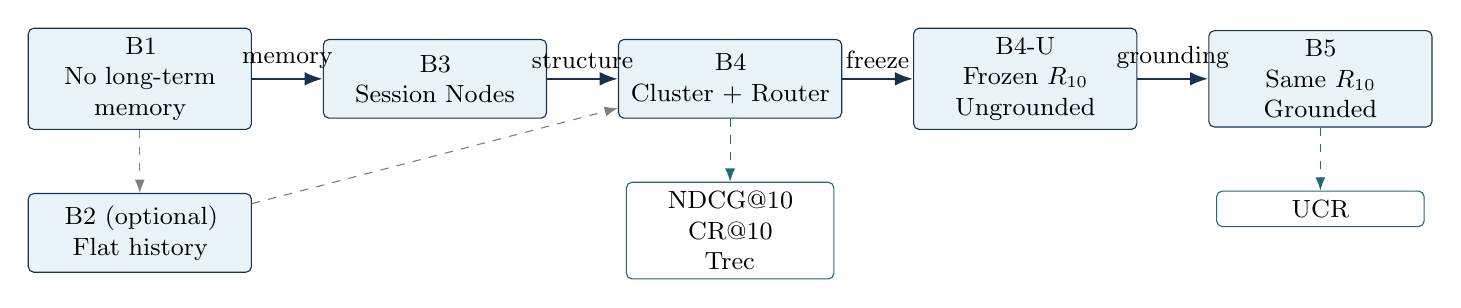
\begin{tikzpicture}[font=\small,node distance=6mm and 9mm,>=Latex,
cond/.style={draw=Navy,rounded corners=2pt,fill=LightBlue,minimum height=10mm,align=center,text width=26mm},
metric/.style={draw=Teal,rounded corners=2pt,fill=white,align=center,text width=24mm},
arr/.style={->,thick,draw=Navy}]
\node[cond] (b1) {B1\\No long-term memory};
\node[cond,right=of b1] (b3) {B3\\Session Nodes};
\node[cond,right=of b3] (b4) {B4\\Cluster + Router};
\node[cond,right=of b4] (u) {B4-U\\Frozen $R_{10}$\\Ungrounded};
\node[cond,right=of u] (b5) {B5\\Same $R_{10}$\\Grounded};
\draw[arr] (b1)-- node[above]{memory} (b3);
\draw[arr] (b3)-- node[above]{structure} (b4);
\draw[arr] (b4)-- node[above]{freeze} (u);
\draw[arr] (u)-- node[above]{grounding} (b5);
\node[metric,below=8mm of b4] (m1) {NDCG@10\\CR@10\\Trec};
\node[metric,below=8mm of b5] (m2) {UCR};
\draw[->,dashed,draw=Teal] (b4)--(m1); \draw[->,dashed,draw=Teal] (b5)--(m2);
\node[cond,below=8mm of b1] (b2) {B2 (optional)\\Flat history};
\draw[->,dashed,draw=gray] (b1)--(b2); \draw[->,dashed,draw=gray] (b2)--(b4);
\end{tikzpicture}
\caption{Core 평가 경로. cross-encoder와 이미지 인덱스는 주 사슬에서 제거했다.}
\label{fig:ladder}
\end{figure*}

\subsection{네 핵심 지표}
\paragraph{NDCG@10.} 작품 적합도 $g_i\in\{0,1,2,3\}$로 개인화 순위를 평가한다\cite{jarvelin2002ndcg}.
\begin{equation}
\mathrm{NDCG}@K=\frac{1}{\mathrm{IDCG}@K}\sum_{i=1}^{K}\frac{2^{g_i}-1}{\log_2(i+1)}.
\end{equation}
관람 가능성은 적합도 등급에 넣지 않고 별도 축으로 유지한다.

\paragraph{CR@10.} 현재 맥락 $c$의 관련 집합을 $P_c$, 다른 맥락들의 합집합을 $P_{\bar c}$라 할 때,
\begin{equation}
\mathrm{CR}@K=\frac{1}{K}\left|\{a\in R_K: a\in P_{\bar c}\setminus P_c\}\right|.
\end{equation}
두 맥락 모두에 적합한 작품은 오염으로 세지 않는다.

\paragraph{Trec.} 취향 전환 이후 CR@10$\le 0.10$이고 새 취향 Recall@10이 Oracle 대비 90\% 이상인 상태가 2턴 연속 유지되는 최초 시점까지의 누적 턴 수로 정의한다. 관찰 기간 내 회복하지 못한 경우 중도절단 여부와 요약 방식을 명시한다.

\paragraph{UCR.} 방문 주장 집합을 $C_{visit}$, grounding record $\Gamma_t$가 claim $\ell$을 지지하는지 여부를 $\mathrm{supp}(\ell,\Gamma_t)$라 하면,
\begin{equation}
\mathrm{UCR}=\frac{|\{\ell\in C_{visit}: \neg\mathrm{supp}(\ell,\Gamma_t)\}|}{|C_{visit}|}.
\end{equation}
주장을 아예 하지 않아 UCR을 낮추는 현상을 막기 위해 verified claim coverage를 보조로 기록한다.

\subsection{통계 분석 계획}
분석 단위는 사용자이다. 동일 사용자·동일 질의·동일 seed·동일 snapshot의 paired design을 유지한다. 실제 평가가 S2(30명의 시뮬레이션 사용자, 300 세션)를 충족하면 사용자 단위 paired cluster bootstrap(예: 10,000회)로 95\% CI를 보고하고, 사전 지정 확증 가설 수에 따라 Holm 보정을 적용한다\cite{efron1993bootstrap,holm1979}. S0/S1 규모에서는 p-value 중심 해석을 피하고 paired difference, CI, 효과크기, 오류 사례를 탐색적으로 보고한다.

\subsection{파인튜닝 조건부 실험}
SFT는 Core의 주 절제 사슬과 분리한다. F0와 F1에서 사용하는 memory/retrieval/grounding을 동일하게 고정하고, Extractor만 변경한다.
\begin{table}[H]
\centering
\caption{조건부 fine-tuning 평가.}
\small
\begin{tabularx}{\columnwidth}{@{}p{0.30\columnwidth}X@{}}
\toprule
항목 & 보고값 \\
\midrule
Explicit extraction & micro-F1 \\
Implicit extraction & micro-F1 \\
Evidence span & token IoU / span accuracy \\
Structure output & JSON validity, required-field success \\
운영 & latency, token/API cost \\
\bottomrule
\end{tabularx}
\end{table}
F1은 F0 대비 실질적인 오류 감소가 있고, 데이터 제작·학습 비용이 전체 일정에 부담되지 않는 경우에만 Core 데모에 채택한다.

\section{결과 및 논의 - 입력 템플릿}
\StatusBox{이 절의 빈칸은 반드시 실제 실행 결과로만 채운다. 목표치, 개발 세트 수치, 예시 숫자를 최종 결과처럼 사용하지 않는다.}

\subsection{Core 결과}
\begin{table*}[t]
\centering
\caption{Core 핵심 결과. 모든 값은 실제 평가 실행 후 입력한다.}
\label{tab:results}
\small
\begin{tabularx}{0.96\textwidth}{@{}p{0.13\textwidth}p{0.15\textwidth}p{0.15\textwidth}p{0.12\textwidth}p{0.18\textwidth}X@{}}
\toprule
Metric & Baseline & ARTHÉMIS-Core & $\Delta$ & 95\% CI / Audit & 해석 \\
\midrule
NDCG@10 $\uparrow$ & \Measured & \Measured & \Measured & \Measured & 개인화 순위 품질 \\
CR@10 $\downarrow$ & \Measured & \Measured & \Measured & \Measured & 맥락 오염 \\
Trec $\downarrow$ & \Measured turns & \Measured turns & \Measured & \Measured & 취향 전환 회복 \\
UCR $\downarrow$ & \Measured & \Measured & \Measured & claim audit \Measured & 미검증 방문 주장 \\
\bottomrule
\end{tabularx}
\end{table*}

\subsection{RQ별 서술 템플릿}
\paragraph{RQ1.} B1과 B4의 사용자 단위 NDCG@10 차이는 \inputslot{DELTA} (95\% CI \inputslot{LOW}, \inputslot{HIGH})였다. 이 결과는 \inputslot{S0/S1/S2} 규모에서 관찰되었으며, \TODO{확증 또는 탐색적 해석을 실제 표본 규모에 맞게 선택}.

\paragraph{RQ2.} B4의 CR@10은 \inputslot{VALUE}였고 비교 조건의 CR@10은 \inputslot{VALUE}였다. 취향 전환 persona의 Trec은 각각 \inputslot{VALUE}와 \inputslot{VALUE} turns였다. 실패 사례는 query\_id \inputslot{IDs}에서 주로 \inputslot{ROOT CAUSE}로 나타났다.

\paragraph{RQ3.} 동일한 $R_{10}$을 고정한 상태에서 B4-U와 B5의 UCR은 각각 \inputslot{VALUE}, \inputslot{VALUE}였다. unsupported claim의 유형은 \inputslot{DATE/VENUE/FEE/STATUS}에 집중되었다.

\paragraph{RQ-FT (조건부).} F0가 사전 지정 extractor 기준을 충족하여 SFT를 수행하지 않았다 / F1을 수행한 결과 explicit F1 \inputslot{}, implicit F1 \inputslot{}, evidence span \inputslot{}, JSON validity \inputslot{}로 나타났다. \TODO{둘 중 실제 경로 하나만 남길 것}.

\subsection{오류 분석}
각 실패는 query\_id, stage, expected, observed, root cause, fix, commit으로 감사 로그와 연결한다. 최소 네 범주를 유지한다: extraction error, memory routing error, retrieval error, grounding/claim error.

\section{구현·재현성과 6주 실행계획}
\subsection{실행 환경과 기록}
최종 원고에는 다음을 채운다: 코퍼스 snapshot/checksum, 전시 API 기준일, \EmbeddingModel, \HostedLLM, prompt\_version, BM25/RRF 파라미터, router threshold, temperature, seed, requirements lock, \GitCommit. 실험의 raw log는 \texttt{audits/}에 보존한다.

\begin{lstlisting}[caption={권고 repository 구조}]
arthemis-core/
  data/{raw,processed,snapshots}/
  src/{ingest,retrieval,memory,grounding,generation}/
  eval/{labels,metrics.py,run_b1.py,run_memory_eval.py,run_grounding_eval.py}
  app/streamlit_app.py
  configs/  audits/  tests/
  requirements.lock  README.md
\end{lstlisting}

\subsection{6주 로드맵}
\begin{table*}[t]
\centering
\caption{다운사이징 반영 6주 실행계획.}
\small
\begin{tabularx}{0.97\textwidth}{@{}p{0.05\textwidth}p{0.16\textwidth}X p{0.25\textwidth}p{0.20\textwidth}@{}}
\toprule
주차 & 목표 & 필수 산출물 & Go 기준 & 실패 시 축소 \\
\midrule
W1 & 데이터/snapshot & artworks, exhibitions, schema audit & E2E 데이터 로딩 + 수동 점검 & 단일 기관·필드 축소 \\
W2 & B1 + Extractor & BM25/dense/RRF, JSON extractor & 20 질의 무중단 + NDCG 코드 실행 & AAT/암묵 슬롯 일부 축소 \\
W3 & Memory & Session Node, Cluster, Router, S0 45 sessions & CR/Trec 자동 계산 & BRIDGE/decay 생략 \\
W4 & Grounding & API adapter, B4-U/B5 & 동일 $R_{10}$에서 UCR audit & 전시 API 1개, 작품단위 주장 금지 \\
W5 & 통제 실험 & B1/B2/B3/B4/B5 반복 & 네 결과칸 + CI/오류 로그 & 이미지/reranker 완전 제외 \\
W6 & 데모/문서 & Streamlit, GitHub, 1분 영상, 포스터 & fresh clone 실행 + 데모 완료 & 캐시 기반 읽기전용 데모 \\
\bottomrule
\end{tabularx}
\end{table*}

\subsection{Go/No-Go 규칙}
새 기능을 추가하기 전 ``이 기능이 NDCG/CR/Trec/UCR 중 무엇을 바꾸는가?'', ``다음 주 실험을 막는 blocker인가?'', ``새 모델/데이터 없이 해결 가능한가?''를 확인한다. B1이 실행되지 않으면 memory/fine-tuning을 추가하지 않는다. CR이 높으면 router를, Trec이 길면 tentative cluster와 확인 질문을, UCR이 높으면 claim constraint를 먼저 수정한다. NDCG만 낮을 때에만 reranker/이미지 인덱스를 검토한다.

\section{한계와 윤리}
첫째, 45/90 세션은 확증 통계보다 파이프라인과 오류 패턴 검증에 적합하다. 둘째, 단일 기관 작품 코퍼스는 외적 타당성을 제한하지만 데이터 통합 변수를 통제한다. 셋째, 전시 단위 API는 원작의 실제 전시 여부를 항상 보장하지 않으므로 관련 전시가 확인되었다는 수준으로만 표현한다. 넷째, 정서 관련 원문은 그대로 장기 저장하지 않고 감상 목적 수준으로 추상화하며 consent scope와 보존기간을 둔다. 다섯째, 근현대 작품 이미지는 기관 이용조건을 따르고 Core에서는 원본 이미지 저장·재배포를 필수로 하지 않는다. 실관람객 파일럿은 IRB 심의 또는 면제 확인과 동의를 전제로 한다.

\section{결론}
본 중간 논문은 ARTHÉMIS의 초기 이상형 설계를 6주 안에 실측 가능한 \ProjectName으로 축소한다. 핵심은 모델 수가 아니라 귀속 가능성이다. 동일 검색기에서 memory만 바꾸어 NDCG/CR/Trec를 측정하고, 동일 추천목록에서 grounding만 바꾸어 UCR을 측정한다. 파인튜닝은 Extractor의 반복 오류가 확인된 경우에만 국소적으로 적용한다. 최종 제출의 성공 조건은 작동하는 데모, 재현 가능한 코드, 네 실측 지표, 실패 사례이며, 이미지 정밀검색·cross-encoder·다기관 확장은 이 조건 이후의 후속 연구로 둔다.

\appendix
\section{제출 직전 값 입력 체크리스트}
\begin{table*}[H]
\centering
\small
\begin{tabularx}{0.97\textwidth}{@{}p{0.23\textwidth}X p{0.23\textwidth}@{}}
\toprule
범주 & 입력 항목 & 상태 \\
\midrule
데이터 & \CorpusName, \ArtworkN, \ExhibitionN, \SnapshotDate, checksum & \TODO{입력} \\
모델 & \EmbeddingModel, \HostedLLM, SFT 사용 여부/모델 ID & \TODO{입력} \\
실험 & 실제 세션 규모 \EvalScale, 개발/평가 분할, seed & \TODO{입력} \\
결과 & NDCG@10, CR@10, Trec, UCR, CI, 오류 사례 & \TODO{입력} \\
재현성 & \GitCommit, requirements.lock, prompt version, audit path & \TODO{입력} \\
윤리 & 라이선스, consent scope, IRB/면제 상태(파일럿 시) & \TODO{입력} \\
\bottomrule
\end{tabularx}
\end{table*}

\section{논문 구조 변경 기록}
\begin{table*}[H]
\centering
\caption{초기 중간논문에서 Core 뼈대로의 구조 변경.}
\small
\begin{tabularx}{0.97\textwidth}{@{}p{0.20\textwidth}p{0.27\textwidth}X@{}}
\toprule
축 & 초기 설계 & Core 재작성 \\
\midrule
검색 & T/X/V/L + reranker & BM25 + text embedding + RRF; 이미지/reranker 옵션 \\
데이터 & 국내외 다기관 & 작품 1개 핵심 코퍼스 + 전시 API 1개 \\
LLM & 복수 역할/모델 가능 & hosted LLM 1종 + 역할별 prompt/schema \\
메모리 & BRIDGE/decay까지 전체 상태기계 & Session Node + Cluster + Router 최소판 \\
그라운딩 & 작품/전시 정합 + availability filtering & 동일 $R_{10}$의 claim grounding을 먼저 검증 \\
평가 & B0--B5 전체, 7 confirmatory hypotheses & NDCG/CR/Trec/UCR 4개 핵심; 표본 규모에 따라 exploratory/confirmatory 구분 \\
파인튜닝 & 역할별 FT 가능성 & Extractor 병목 시에만 optional SFT \\
\bottomrule
\end{tabularx}
\end{table*}

\section{최소 실행 명령}
\begin{lstlisting}
python eval/run_b1.py
# -> NDCG@10, Recall@50, MRR

python eval/run_memory_eval.py
# -> NDCG@10, CR@10, Trec

python eval/run_grounding_eval.py
# -> UCR, verified claim coverage, claim audit

streamlit run app/streamlit_app.py
# -> input -> memory -> recommendation -> exhibition status
\end{lstlisting}

\balance
\begin{thebibliography}{99}\small
\bibitem{achlioptas2021artemis} P. Achlioptas, M. Ovsjanikov, K. Haydarov, M. Elhoseiny, and L. Guibas. ArtEmis: Affective language for visual art. \textit{CVPR}, 2021.
\bibitem{cormack2009rrf} G. V. Cormack, C. L. A. Clarke, and S. Buettcher. Reciprocal rank fusion outperforms Condorcet and individual rank learning methods. \textit{SIGIR}, 2009.
\bibitem{efron1993bootstrap} B. Efron and R. J. Tibshirani. \textit{An Introduction to the Bootstrap}. Chapman \& Hall, 1993.
\bibitem{friedman2023recllm} L. Friedman et al. Leveraging large language models in conversational recommender systems. arXiv:2305.07961, 2023.
\bibitem{holm1979} S. Holm. A simple sequentially rejective multiple test procedure. \textit{Scandinavian Journal of Statistics}, 1979.
\bibitem{jannach2021crs} D. Jannach, A. Manzoor, W. Cai, and L. Chen. A survey on conversational recommender systems. \textit{ACM Computing Surveys}, 54(5), 2021.
\bibitem{jarvelin2002ndcg} K. J\"arvelin and J. Kek\"al\"ainen. Cumulated gain-based evaluation of IR techniques. \textit{ACM TOIS}, 20(4), 2002.
\bibitem{maharana2024locomo} A. Maharana et al. Evaluating very long-term conversational memory of LLM agents. \textit{ACL}, 2024.
\bibitem{wu2025longmemeval} D. Wu et al. LongMemEval: Benchmarking chat assistants on long-term interactive memory. \textit{ICLR}, 2025.
\bibitem{xu2025amem} W. Xu et al. A-MEM: Agentic memory for LLM agents. arXiv:2502.12110, 2025.
\end{thebibliography}

\end{document}
